% Cuando se desarrolla una idea de un prototipo, se necesita una sección donde listar los distintos componentes hardware o software que se utilizará en el proceso de investigación.
% En los componentes hardware normalmente se encuentran los sensores. Los componentes software están más orientados a la arquitectura y
% al diseño de las aplicaciones, y no a los framework y lenguaje utilizados.

\begin{figure}[htbp]
    \centering
    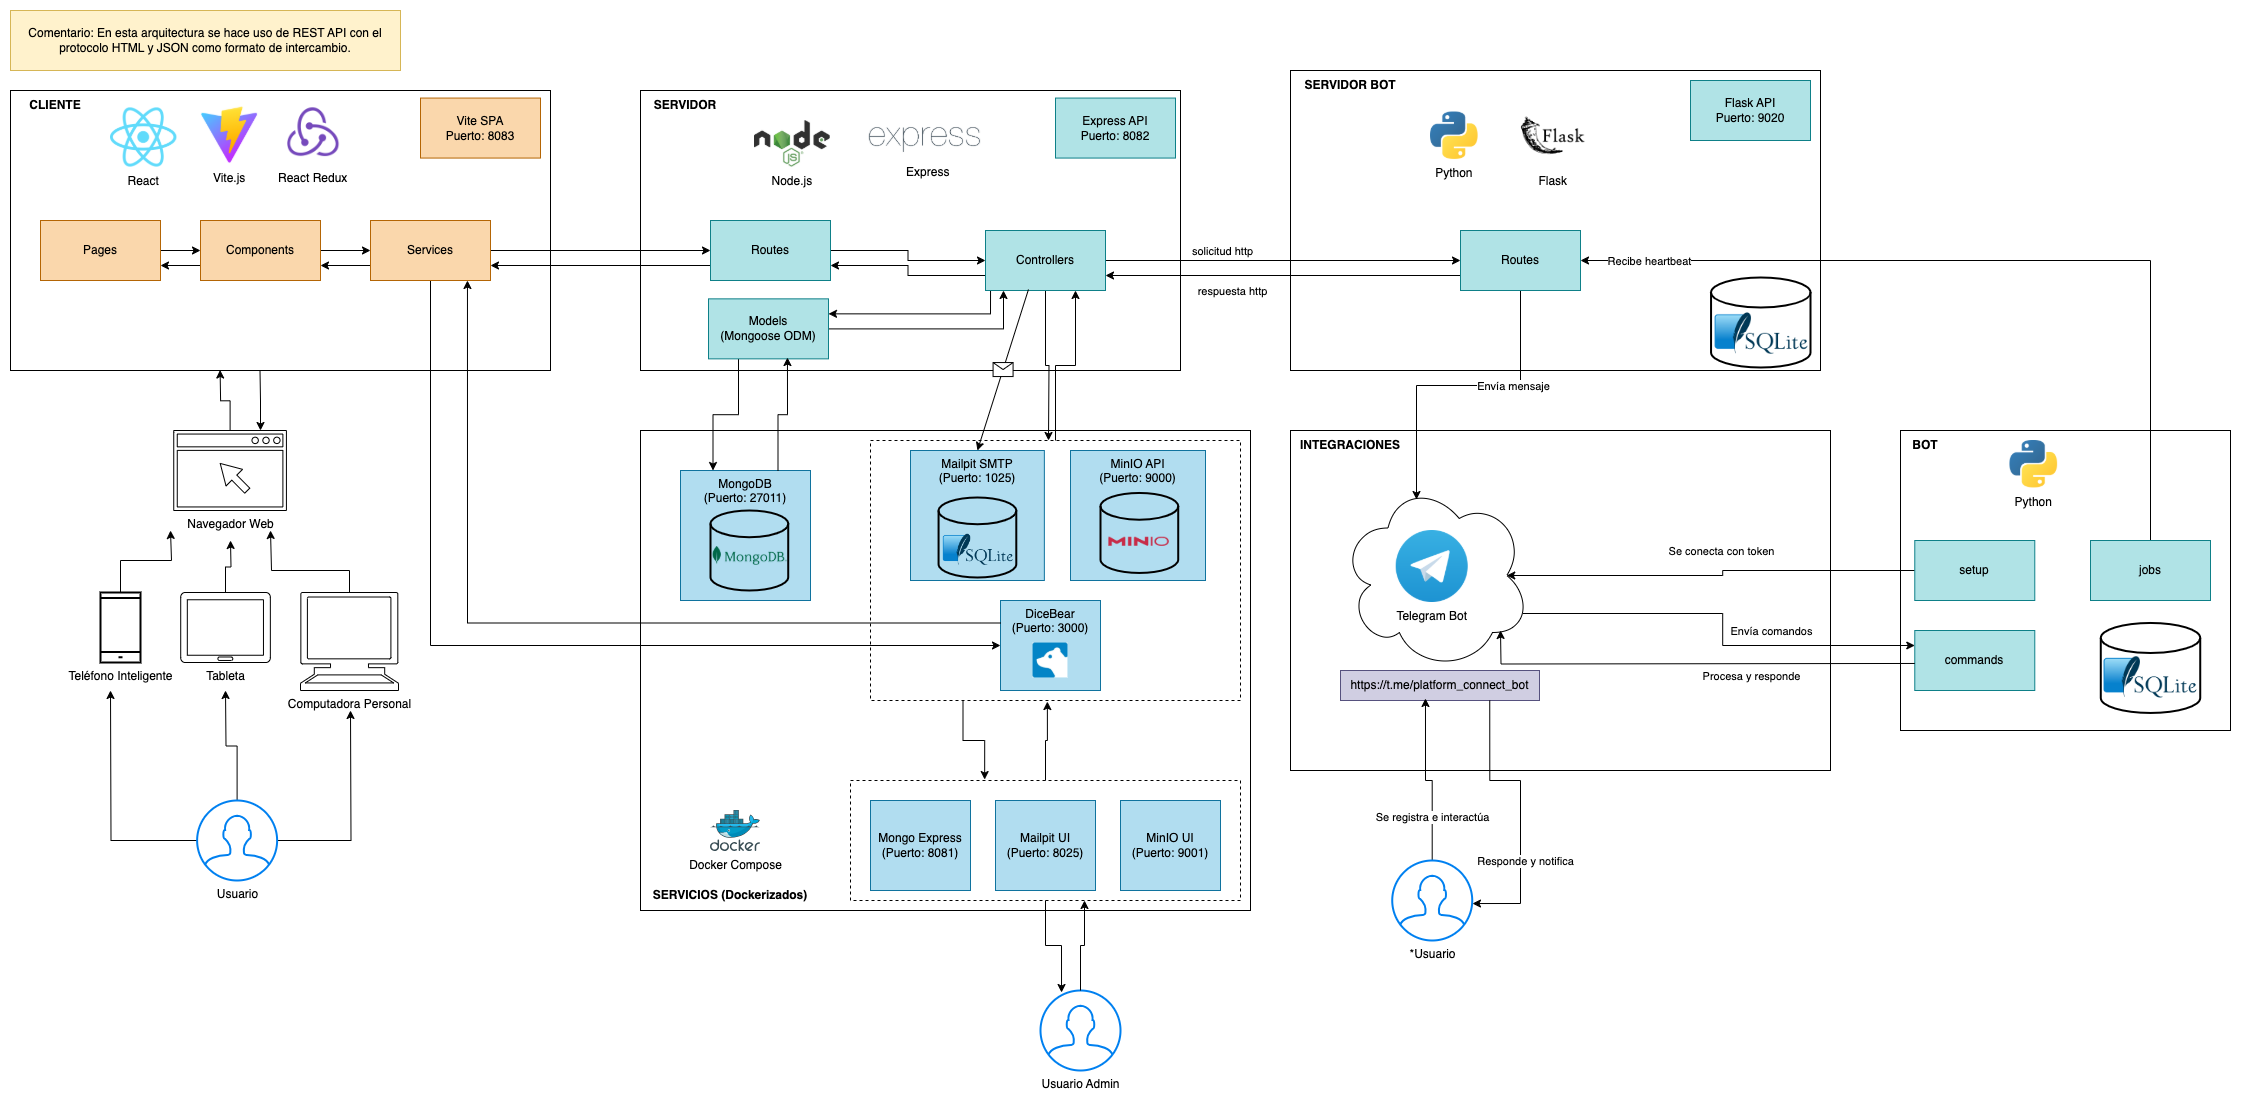
\includegraphics[width=\linewidth]{diagrama_arquitectura/diagrama_arquitectura.png}
    \caption{Arquitectura General del Sistema}
    \label{fig:diagrama_arquitectura}
\end{figure}

La Figura \ref{fig:diagrama_arquitectura} presenta la arquitectura general de la
solución propuesta. El sistema está compuesto por seis elementos principales: el
bot, el cliente, las integraciones, los servicios backend, el servidor y el
servidor bot. 

La interacción principal ocurre cuando los usuarios acceden a la solución
desde un navegador web. A partir de esta interacción, las solicitudes son
procesadas por el cliente, que luego se comunica con el servidor y los servicios
asociados para garantizar una experiencia fluida.

\begin{figure}[htbp]
    \centering
    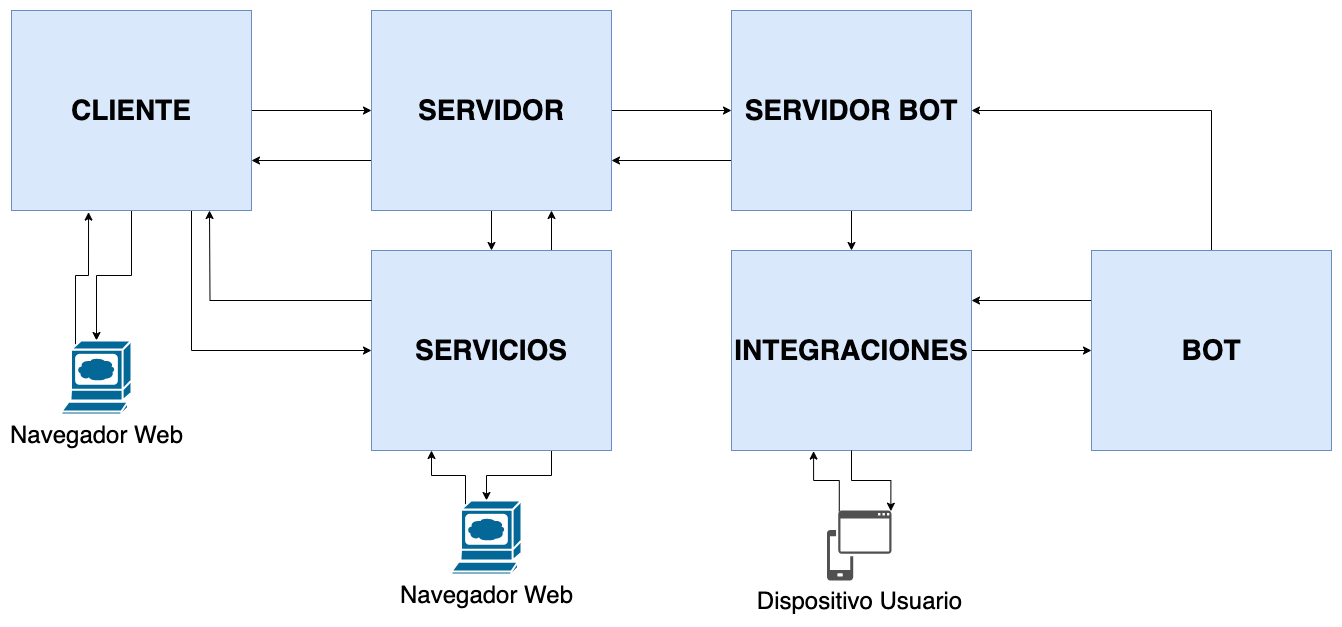
\includegraphics[width=\linewidth]{diagrama_arquitectura/diagrama_arquitectura_alto_nivel.png}
    \caption{Arquitectura del Sistema - Vista de Alto Nivel}
    \label{fig:diagrama_arquitectura_alto_nivel}
\end{figure}

La Figura \ref{fig:diagrama_arquitectura_alto_nivel} ilustra la arquitectura a
un nivel más abstracto, proporcionando una visión general de los distintos
módulos que conforman el sistema. Este enfoque permite identificar las
principales áreas funcionales sin entrar en los detalles internos de cada
componente. 

Este diagrama facilita la comprensión de la interacción entre los elementos
clave del sistema, ayudando a visualizar cómo se conectan entre sí para
garantizar el funcionamiento eficiente de la solución.

\begin{figure}[htbp]
    \centering
    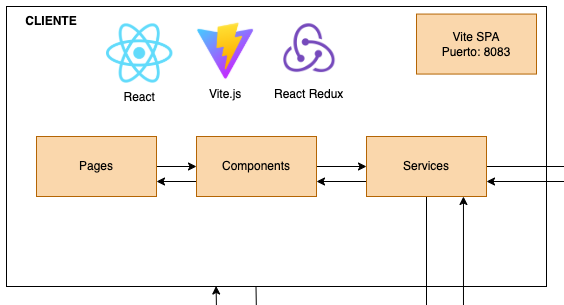
\includegraphics[width=\linewidth]{diagrama_arquitectura/diagrama_arquitectura_cliente.png}
    \caption{Arquitectura del Cliente}
    \label{fig:diagrama_arquitectura_cliente}
\end{figure}

La Figura \ref{fig:diagrama_arquitectura_cliente} muestra la arquitectura del
cliente, que constituye la interfaz de usuario y su comunicación con el
servidor. Este módulo ha sido desarrollado en \textbf{React} y permite una
interacción dinámica entre el usuario y el sistema, garantizando una experiencia
fluida y adaptativa.

El cliente cumple las siguientes funciones principales:
\begin{itemize}
    \item Renderizar la interfaz gráfica y gestionar el estado de la aplicación.
    \item Procesar la navegación y las interacciones del usuario.
    \item Enviar solicitudes al servidor mediante API REST y procesar las
    respuestas para actualizar el contenido educativo en tiempo real.
\end{itemize}

Además, la implementación se ha basado en la guía oficial de
\href{https://vite.dev/guide/}{Vite}, optimizando el rendimiento y el proceso de
desarrollo del frontend.

\begin{figure}[htbp]
    \centering
    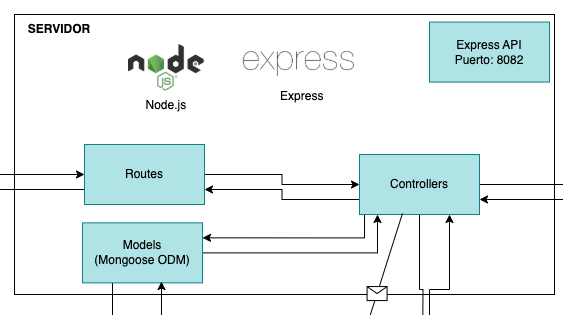
\includegraphics[width=\linewidth]{diagrama_arquitectura/diagrama_arquitectura_servidor.png}
    \caption{Arquitectura del Servidor}
    \label{fig:diagrama_arquitectura_servidor}
\end{figure}

La Figura \ref{fig:diagrama_arquitectura_servidor} representa la arquitectura
del \textbf{servidor backend}, diseñado en \textbf{Node.js} con el framework
\textbf{Express} para gestionar la lógica del sistema y coordinar la interacción
con los servicios backend.

Las principales responsabilidades del servidor incluyen:
\begin{itemize}
    \item Autenticación y autorización de usuarios mediante JWT o OAuth.
    \item Manejo de solicitudes provenientes del cliente y distribución de
    respuestas adecuadas.
    \item Comunicación eficiente con los servicios en contenedores Docker, como
    \textbf{MongoDB}, \textbf{MinIO}, \textbf{Mailpit}, \textbf{Mongo Express} y
    \textbf{DiceBear}.
    \item Administración de la infraestructura de almacenamiento y procesamiento
    de datos, garantizando disponibilidad y escalabilidad.
\end{itemize}

Este servidor actúa como el núcleo de la solución, proporcionando una capa
intermedia entre el frontend y los servicios backend, asegurando la integridad y
consistencia de la información dentro del sistema LMS basado en microlearning.

\begin{figure}[htbp]
    \centering
    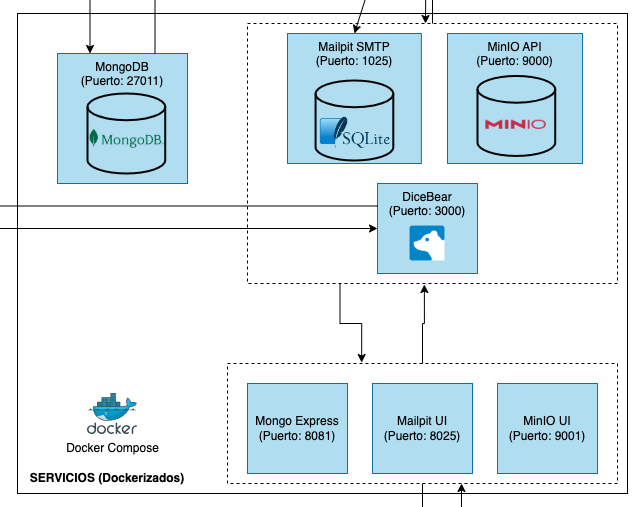
\includegraphics[width=\linewidth]{diagrama_arquitectura/diagrama_arquitectura_servicios.png}
    \caption{Arquitectura de los Servicios Backend}
    \label{fig:diagrama_arquitectura_servicios}
\end{figure}

La Figura \ref{fig:diagrama_arquitectura_servicios} muestra los servicios
backend desplegados en contenedores Docker para garantizar escalabilidad, portabilidad y
facilidad de mantenimiento dentro del sistema. Estos servicios operan de manera
independiente, permitiendo una gestión eficiente de datos y recursos.

Entre los principales servicios se incluyen:
\begin{itemize}
    \item \textbf{MongoDB}: Base de datos NoSQL utilizada para almacenar
    información de usuarios, cursos y progreso en el aprendizaje.
    \item \textbf{Mongo Express}: Interfaz web que permite la administración
    visual de la base de datos MongoDB de manera intuitiva.
    \item \textbf{MinIO (API + WebUI)}: Plataforma de almacenamiento de objetos
    compatible con S3, utilizada para gestionar archivos y recursos educativos.
    \item \textbf{Mailpit (SMTP + WebUI)}: Servicio de correo electrónico que
    facilita la entrega de notificaciones y la administración de correos
    generados por el sistema.
    \item \textbf{DiceBear}: Generador de avatares dinámicos que mejora la
    personalización visual de los perfiles de usuario.
\end{itemize}

Estos servicios, junto con el \textbf{bot} y el \textbf{bot server}, han sido
configurados para ejecutarse dentro de contenedores Docker, proporcionando un
entorno modular y eficiente. Además, las interfaces de \textbf{MinIO},
\textbf{Mailpit} y \textbf{Mongo Express} están accesibles para usuarios
administradores, lo que permite una gestión optimizada de los datos y archivos
dentro del sistema.

\begin{figure}[htbp]
    \centering
    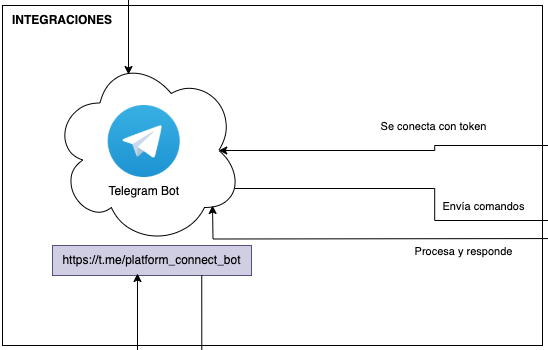
\includegraphics[width=\linewidth]{diagrama_arquitectura/diagrama_arquitectura_integraciones.png}
    \caption{Arquitectura de Integraciones Externas}
    \label{fig:diagrama_arquitectura_integraciones}
\end{figure}

La Figura \ref{fig:diagrama_arquitectura_integraciones} muestra las
integraciones externas que enriquecen la funcionalidad del sistema LMS. Si bien
la implementación actual está centrada en la integración con Telegram, la
arquitectura ha sido diseñada para permitir futuras extensiones hacia otras
plataformas. Estas integraciones buscan mejorar la experiencia del usuario,
facilitar la automatización de tareas y proporcionar canales adicionales de
acceso al contenido educativo.

\begin{figure}[htbp]
    \centering
    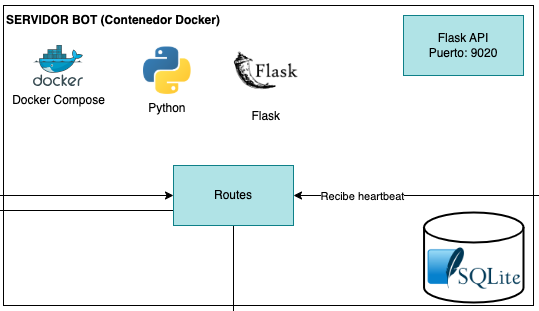
\includegraphics[width=\linewidth]{diagrama_arquitectura/diagrama_arquitectura_servidor_bot.png}
    \caption{Arquitectura del Servidor Bot}
    \label{fig:diagrama_arquitectura_servidor_bot}
\end{figure}

La Figura \ref{fig:diagrama_arquitectura_servidor_bot} representa la
arquitectura del \textbf{Servidor Bot}, que actúa como intermediario entre el
sistema LMS y la integración con Telegram. Este componente, desarrollado en
\textbf{Python} utilizando \textbf{Flask}, recibe y procesa solicitudes del
cliente, enviando respuestas adecuadas al bot. Su diseño modular permite la
adaptación a futuras integraciones con otros servicios de mensajería.

\begin{figure}[htbp]
    \centering
    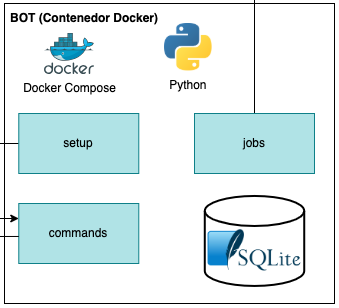
\includegraphics[width=\linewidth]{diagrama_arquitectura/diagrama_arquitectura_bot.png}
    \caption{Arquitectura del Bot de Mensajería}
    \label{fig:diagrama_arquitectura_bot}
\end{figure}

La Figura \ref{fig:diagrama_arquitectura_bot} muestra el \textbf{Bot de
Telegram}, desarrollado en \textbf{Python}, que facilita el acceso al contenido
de microlearning directamente desde la plataforma de mensajería.
Al momento de esta investigación, la integración ofrecen notificaciones sobre nuevos contenidos.
Se espera poder expandir sus funcionalidades a futuro para incluir:
\begin{itemize}
    \item Envío de recordatorios sobre contenido.
    \item Continuar mejorando el acceso rápido a recursos educativos.
\end{itemize}

Si bien la implementación inicial está enfocada en Telegram, el diseño de este
bot permite su extensión a otras plataformas de mensajería, asegurando
flexibilidad y adaptabilidad en futuras versiones del sistema LMS.





